\documentclass[aspectratio=169]{beamer}

\usetheme{Boadilla}
\usefonttheme{professionalfonts}
\setbeamertemplate{navigation symbols}{}
\setbeamertemplate{itemize items}[circle]
\setbeamertemplate{enumerate items}[default]
\setbeamertemplate{headline}{}

\usepackage[utf8]{inputenc}
\usepackage[T1]{fontenc}
\usepackage{lmodern}
\usepackage{amsmath}
\usepackage{booktabs}
\usepackage{tabularx}
\usepackage{array}
\usepackage{hyperref}
\usepackage[strings]{underscore}
\usepackage{listings}
\usepackage{tikz}
\usetikzlibrary{arrows.meta,positioning,fit,calc,shapes.geometric}
\usepackage{xcolor}

\definecolor{courseblue}{HTML}{12355B}
\definecolor{coursegold}{HTML}{C98A2E}
\definecolor{courseice}{HTML}{EEF3F8}
\definecolor{coursegreen}{HTML}{2F6B4F}
\definecolor{coursegray}{HTML}{4B5563}
\definecolor{codebg}{HTML}{F7F9FC}
\definecolor{codecomment}{HTML}{5E6C84}
\definecolor{codestring}{HTML}{0B6E4F}

\setbeamercolor{palette primary}{bg=courseblue,fg=white}
\setbeamercolor{palette secondary}{bg=coursegold,fg=white}
\setbeamercolor{palette tertiary}{bg=courseblue,fg=white}
\setbeamercolor{palette quaternary}{bg=coursegold,fg=white}
\setbeamercolor{structure}{fg=courseblue}
\setbeamercolor{frametitle}{bg=courseice,fg=courseblue}
\setbeamercolor{title}{fg=courseblue}
\setbeamercolor{block title}{bg=courseblue,fg=white}
\setbeamercolor{block body}{bg=courseice,fg=black}
\setbeamercolor{normal text}{fg=black,bg=white}
\setbeamercolor{alerted text}{fg=coursegold}

\setbeamerfont{footline}{size=\scriptsize}

\setbeamertemplate{footline}{
  \leavevmode
  \hbox{
    \begin{beamercolorbox}[wd=.33\paperwidth,ht=2.8ex,dp=1.2ex,leftskip=0.8em]{palette primary}%
      University of Trieste
    \end{beamercolorbox}%
    \begin{beamercolorbox}[wd=.49\paperwidth,ht=2.8ex,dp=1.2ex,center]{palette tertiary}%
      \coursename{} \textbar{} \coursecode
    \end{beamercolorbox}%
    \begin{beamercolorbox}[wd=.18\paperwidth,ht=2.8ex,dp=1.2ex,rightskip=0.8em plus1fil]{palette secondary}%
      \insertframenumber{} / \inserttotalframenumber
    \end{beamercolorbox}%
  }
}

\hypersetup{
  colorlinks=true,
  linkcolor=courseblue,
  urlcolor=coursegreen
}

\lstdefinestyle{coursepython}{
  language=Python,
  basicstyle=\ttfamily\footnotesize,
  keywordstyle=\color{courseblue}\bfseries,
  commentstyle=\color{codecomment}\itshape,
  stringstyle=\color{codestring},
  showstringspaces=false,
  columns=fullflexible,
  keepspaces=true,
  frame=single,
  framerule=0.6pt,
  rulecolor=\color{courseblue},
  backgroundcolor=\color{codebg},
  xleftmargin=0.4em,
  xrightmargin=0.4em,
  aboveskip=0.4em,
  belowskip=0.2em
}

\newcommand{\coursename}{Data-driven Systems Engineering}
\newcommand{\coursecode}{440MI / 305SM}
\newcommand{\coursefooter}{}

\newcommand{\learninggoals}[1]{
  \begin{block}{Learning goals}
  #1
  \end{block}
}

\newcommand{\repoactivity}[1]{
  \begin{block}{Repo activity}
  #1
  \end{block}
}

\newcommand{\readinglist}[1]{
  \begin{block}{Papers and materials}
  {\footnotesize #1}
  \end{block}
}

\newcommand{\coursecontextframe}[5]{
  \begin{frame}{Course Map and Running Cases}
  \centering
  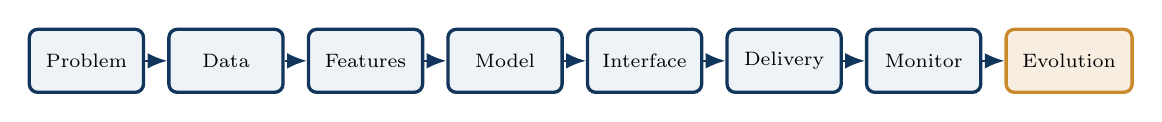
\begin{tikzpicture}[node distance=0.28cm]
  \node[flowbox, minimum width=1.45cm, minimum height=0.8cm] (problem) {\scriptsize Problem};
  \node[flowbox, minimum width=1.45cm, minimum height=0.8cm, right=of problem] (data) {\scriptsize Data};
  \node[flowbox, minimum width=1.45cm, minimum height=0.8cm, right=of data] (features) {\scriptsize Features};
  \node[flowbox, minimum width=1.45cm, minimum height=0.8cm, right=of features] (model) {\scriptsize Model};
  \node[flowbox, minimum width=1.45cm, minimum height=0.8cm, right=of model] (interface) {\scriptsize Interface};
  \node[flowbox, minimum width=1.45cm, minimum height=0.8cm, right=of interface] (delivery) {\scriptsize Delivery};
  \node[flowbox, minimum width=1.45cm, minimum height=0.8cm, right=of delivery] (monitor) {\scriptsize Monitor};
  \node[accentbox, minimum width=1.6cm, minimum height=0.8cm, right=of monitor] (evolution) {\scriptsize Evolution};
  \foreach \a/\b in {problem/data,data/features,features/model,model/interface,interface/delivery,delivery/monitor,monitor/evolution} {
    \draw[arrow] (\a) -- (\b);
  }
  \end{tikzpicture}

  \vspace{0.5em}
  \begin{block}{Today in the course}
  \textbf{Focus:} #1

  \textbf{Bridge:} #2
  \end{block}

  \begin{columns}[T]
  \column{0.48\textwidth}
  \begin{block}{Fraud case}
  {\footnotesize #3}
  \end{block}
  \column{0.48\textwidth}
  \begin{block}{Pasteurization case}
  {\footnotesize #4}
  \end{block}
  \end{columns}

  \vspace{0.3em}
  {\footnotesize \textbf{Course thread:} #5}
  \coursefooter
  \end{frame}
}

\newcommand{\classclosingframe}[4]{
  \begin{frame}{From This Class to the Next}
  \begin{block}{What stays with us}
  #1
  \end{block}

  \begin{columns}[T]
  \column{0.48\textwidth}
  \begin{block}{Project use}
  {\footnotesize #2}
  \end{block}
  \column{0.48\textwidth}
  \begin{block}{Next connection}
  {\footnotesize #3}
  \end{block}
  \end{columns}

  \vspace{0.3em}
  {\footnotesize \textbf{Course thread:} #4}
  \coursefooter
  \end{frame}
}

\tikzset{
  flowbox/.style={
    rounded corners=3pt,
    draw=courseblue,
    fill=courseice,
    very thick,
    minimum width=2.2cm,
    minimum height=0.9cm,
    align=center,
    font=\small
  },
  accentbox/.style={
    rounded corners=3pt,
    draw=coursegold,
    fill=coursegold!15,
    very thick,
    minimum width=2.2cm,
    minimum height=0.9cm,
    align=center,
    font=\small
  },
  arrow/.style={
    -{Latex[length=2.5mm,width=2mm]},
    thick,
    draw=courseblue
  }
}

\usepackage{amssymb}

\title{Class 18: Modeling, Experiment Tracking, Evaluation, and Decision-Making}
\author{\coursename}
\date{}


% Roadmap and transition slides
\newcommand{\partstrip}[1]{%
\begin{center}
\begin{tikzpicture}
\foreach \i/\l in {1/Modeling,2/Tracking,3/Registry,4/Evaluation,5/Decisions,6/Practice}{%
  \def\sty{flowbox}\ifnum\i=#1 \def\sty{accentbox}\fi
  \node[\sty, minimum width=1.75cm, minimum height=0.7cm, font=\scriptsize] at ({(\i-1)*1.95},0) {\i.\ \l};
}
\end{tikzpicture}
\end{center}}

\newcommand{\roadmaprow}[3]{%
\node[flowbox, minimum width=0.8cm, minimum height=0.8cm] (n#1) at (0,{-(#1-1)*1.1}) {\textbf{#1}};
\node[flowbox, anchor=west, text width=0.78\textwidth, align=left, minimum height=0.8cm] at ([xshift=0.15cm]n#1.east) {\textbf{#2}\\[-0.1em]{\scriptsize\color{coursegray}#3}};}

\newcommand{\partslide}[4]{%
\begin{frame}{Roadmap: part #1 of 6}
\vfill
\begin{center}
{\LARGE\bfseries\color{courseblue} #2}\\[0.8em]
{\large\itshape #3}\\[0.8em]
{\footnotesize\color{coursegray} #4}
\end{center}
\vfill
\partstrip{#1}
\coursefooter
\end{frame}}


% Question icons and question/answer slides
\newcommand{\qicon}[1]{%
\begin{tikzpicture}[ic/.style={draw=courseblue, thick, line cap=round, line join=round}]
\node[flowbox, minimum width=1.2cm, minimum height=1.1cm] {};
\begin{scope}[scale=0.38]
\ifcase#1\or
\draw[ic] (-1.3,0) -- (-0.3,0);
\draw[ic, -{Latex[length=1.4mm]}] (-0.3,0) -- (0.3,0.9) -- (1.3,0.9);
\draw[ic, -{Latex[length=1.4mm]}, coursegold] (-0.3,0) -- (0.3,-0.9) -- (1.3,-0.9);
\or
\fill[courseblue] (-1.2,0.8) circle (0.3);
\fill[coursegold] (-0.5,0.8) circle (0.3);
\draw[ic] (-1.2,-0.1) -- (1.2,-0.1);
\fill[coursegold] (0.4,-0.1) circle (0.14);
\draw[ic] (-1.2,-1.2) -- (-0.4,-1.0) .. controls (0,-0.4) .. (0.6,-0.9) -- (1.2,-0.5);
\or
\draw[ic] (0,-1.2) -- (0,0.9);
\draw[ic] (-0.6,-1.2) -- (0.6,-1.2);
\draw[ic] (-1.3,0.5) -- (1.3,1.1);
\draw[ic] (-1.3,0.5) -- (-1.6,-0.3) -- (-1.0,-0.3) -- cycle;
\draw[ic, coursegold] (1.3,1.1) -- (1.0,0.3) -- (1.6,0.3) -- cycle;
\or
\draw[ic] (0,0) circle (1.1);
\draw[ic, coursegold] (0,0) -- (0,0.75);
\draw[ic] (0,0) -- (0.55,-0.25);
\draw[ic] (-0.15,1.3) -- (0.15,1.3);
\or
\draw[ic] (-1.4,-1) -- (1.4,-1);
\draw[ic, domain=-1.3:0.5, samples=25, smooth] plot (\x, {-1+1.6*exp(-4*(\x+0.4)*(\x+0.4))});
\draw[ic, coursegold, domain=-0.5:1.3, samples=25, smooth] plot (\x, {-1+1.6*exp(-4*(\x-0.4)*(\x-0.4))});
\fi
\end{scope}
\end{tikzpicture}}

\newcommand{\qaslide}[7]{%
\begin{frame}{Question #1 of 5: #2}
\begin{minipage}[c]{1.5cm}\qicon{#1}\end{minipage}\hfill
\begin{minipage}[c]{0.85\textwidth}\large #3\end{minipage}
\vspace{0.8em}
\begin{columns}[T]
\column{0.49\textwidth}
\begin{block}{A. #4}\small #5\end{block}
\column{0.49\textwidth}
\begin{alertblock}{B. #6}\small #7\end{alertblock}
\end{columns}
\coursefooter
\end{frame}}


% Model family cards
\newcommand{\famicon}[1]{%
\begin{scope}[ic/.style={draw=courseblue, thick, line cap=round, line join=round}]
\ifcase#1\or
% linear
\draw[ic] (-1.2,-0.9) -- (-1.2,0.9); \draw[ic] (-1.2,-0.9) -- (1.2,-0.9);
\foreach \px/\py in {-0.8/-0.5,-0.4/-0.1,-0.1/-0.4,0.2/0.1,0.5/0.2,0.8/0.7}{\fill[courseblue!60] (\px,\py) circle (0.09);}
\draw[ic, coursegold, very thick] (-1.0,-0.7) -- (1.1,0.8);
\or
% tree
\node[circle, fill=courseblue, inner sep=1.6pt] (r) at (0,0.8) {};
\node[circle, fill=courseblue, inner sep=1.6pt] (a) at (-0.7,0) {};
\node[circle, fill=courseblue, inner sep=1.6pt] (b) at (0.7,0) {};
\node[circle, fill=coursegold, inner sep=1.6pt] (c) at (-1.1,-0.8) {};
\node[circle, fill=coursegold, inner sep=1.6pt] (d) at (-0.3,-0.8) {};
\node[circle, fill=coursegold, inner sep=1.6pt] (e) at (0.7,-0.8) {};
\draw[ic] (r)--(a) (r)--(b) (a)--(c) (a)--(d) (b)--(e);
\or
% probabilistic
\draw[ic] (-1.3,-0.9) -- (1.3,-0.9);
\fill[coursegold!35, domain=0.2:1.1, samples=20] (0.2,-0.9) -- plot (\x,{-0.9+1.7*exp(-1.6*\x*\x)}) -- (1.1,-0.9) -- cycle;
\draw[ic, domain=-1.3:1.3, samples=40, smooth] plot (\x,{-0.9+1.7*exp(-1.6*\x*\x)});
\or
% neural network
\foreach \l/\n in {0/3,1/4,2/2}{\foreach \k in {1,...,\n}{\node[circle, fill=courseblue, inner sep=1.5pt] (n\l\k) at ({-1+\l},{(\k-(\n+1)/2)*0.55}) {};}}
\foreach \k in {1,...,3}{\foreach \m in {1,...,4}{\draw[courseblue!40] (n0\k)--(n1\m);}}
\foreach \k in {1,...,4}{\foreach \m in {1,2}{\draw[courseblue!40] (n1\k)--(n2\m);}}
\fill[coursegold] (n21) circle (2pt); \fill[coursegold] (n22) circle (2pt);
\or
% online
\foreach \px in {-1.3,-0.9,-0.5}{\fill[courseblue!60] (\px,0.1) circle (0.1);}
\draw[ic, -{Latex[length=1.6mm]}] (-0.3,0.1) -- (0.1,0.1);
\node[draw=coursegold, very thick, rounded corners=2pt, minimum width=0.9cm, minimum height=0.8cm, inner sep=0] at (0.65,0.1) {};
\draw[ic, coursegold, -{Latex[length=1.6mm]}] (0.2,-0.5) .. controls (0.65,-1.0) .. (1.1,-0.5);
\or
% kernel / margin
\draw[ic, dashed, coursegold] (0,0) circle (0.65);
\foreach \px/\py in {-0.2/0.1,0.15/-0.15,0.1/0.25,-0.25/-0.2}{\fill[courseblue] (\px,\py) circle (0.09);}
\foreach \px/\py in {-1.0/0.6,1.0/0.7,-0.9/-0.7,1.0/-0.6,0/1.0,0.1/-1.0}{\fill[coursegold] (\px,\py) circle (0.09);}
\or
% instance-based (kNN)
\foreach \px/\py in {-1.0/0.6,-0.7/0.2,-1.1/-0.3,-0.6/-0.7,-0.3/0.7}{\fill[courseblue] (\px,\py) circle (0.09);}
\foreach \px/\py in {1.0/0.6,0.8/-0.2,1.1/-0.6,0.5/0.2,0.6/0.8}{\fill[coursegold] (\px,\py) circle (0.09);}
\draw[ic, dashed] (0.1,-0.1) circle (0.7);
\draw[ic, very thick] (0.1,-0.1) circle (0.05);
\or
% clustering
\foreach \px/\py in {-1.0/0.4,-0.7/0.7,-0.8/0.1,-0.5/0.4}{\fill[courseblue] (\px,\py) circle (0.09);}
\foreach \px/\py in {0.5/0.7,0.8/0.4,1.0/0.8,0.7/0.9}{\fill[coursegold] (\px,\py) circle (0.09);}
\foreach \px/\py in {-0.1/-0.7,0.2/-0.9,0.4/-0.6,0.0/-0.4}{\fill[coursegreen] (\px,\py) circle (0.09);}
\draw[courseblue, thick] (-0.75,0.4) ellipse (0.55 and 0.5);
\draw[coursegold, thick] (0.75,0.7) ellipse (0.55 and 0.4);
\draw[coursegreen, thick] (0.15,-0.65) ellipse (0.5 and 0.45);
\or
% dimensionality reduction (PCA)
\foreach \px/\py in {-1.0/-0.6,-0.7/-0.2,-0.4/-0.5,-0.2/0.0,0.1/-0.1,0.3/0.3,0.6/0.2,0.8/0.7,1.0/0.4,-0.5/-0.1,0.4/0.55}{\fill[courseblue!60] (\px,\py) circle (0.08);}
\draw[ic, coursegold, very thick, -{Latex[length=1.8mm]}] (-1.2,-0.8) -- (1.2,0.8);
\or
% anomaly
\foreach \px/\py in {-0.9/-0.3,-0.6/0.0,-0.3/-0.4,-0.1/0.1,0.1/-0.3,0.3/0.0,-0.5/-0.7,0.0/-0.6}{\fill[courseblue] (\px,\py) circle (0.09);}
\fill[coursegold] (0.95,0.75) circle (0.12);
\draw[ic, coursegold] (0.95,0.75) circle (0.32);
\or
% sequence / time series
\draw[ic] (-1.3,-0.8) -- (1.3,-0.8);
\draw[ic] (-1.3,-0.2) .. controls (-0.9,0.7) and (-0.5,0.7) .. (-0.1,0.0) .. controls (0.1,-0.3) and (0.2,-0.2) .. (0.3,0.1);
\draw[ic, coursegold, dashed, -{Latex[length=1.6mm]}] (0.3,0.1) .. controls (0.6,0.8) and (0.9,0.6) .. (1.3,0.3);
\fi
\end{scope}}

\newcommand{\famcard}[7]{%
\node[draw=courseblue!35, fill=courseice, rounded corners=4pt, thick, minimum width=3.65cm, minimum height=3.15cm] at (#1,#2) {};
\begin{scope}[shift={(#1,{#2+0.85})}, scale=0.55]\famicon{#3}\end{scope}
\node[font=\small\bfseries, text=courseblue] at (#1,{#2+0.05}) {#4};
\node[font=\scriptsize, text width=3.3cm, align=center, text=coursegray, anchor=north] at (#1,{#2-0.2}) {#5};
\node[font=\scriptsize\bfseries, text=coursegold] at (#1,{#2-1.2}) {#6};
\node[font=\fontsize{6.5}{7}\selectfont, text=coursegray] at (#1,{#2-1.44}) {#7};}

\newcommand{\hlcode}[1]{\colorbox{coursegold!35}{\bfseries #1}}

\begin{document}

\frame{\titlepage \coursefooter}

\begin{frame}{Roadmap of the class}
\centering
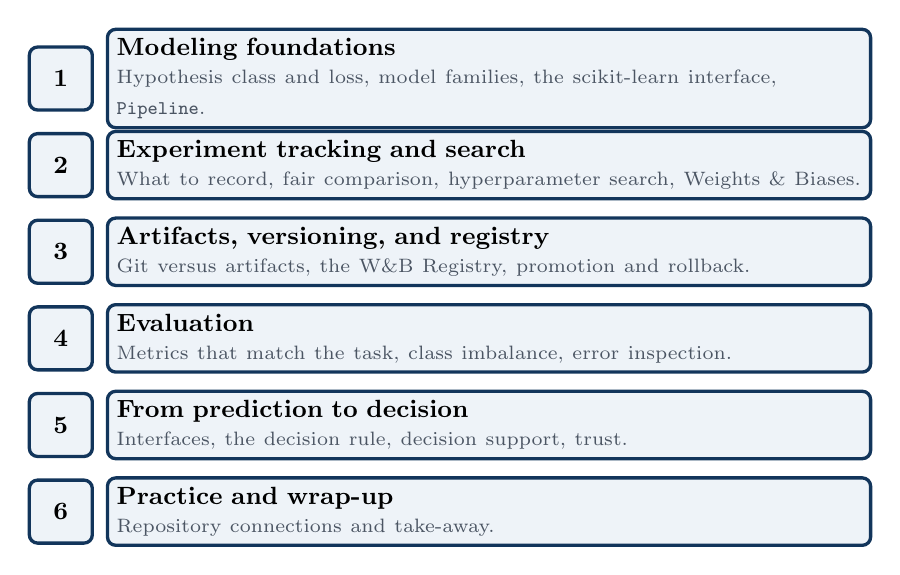
\begin{tikzpicture}
\roadmaprow{1}{Modeling foundations}{Hypothesis class and loss, model families, the scikit-learn interface, \texttt{Pipeline}.}
\roadmaprow{2}{Experiment tracking and search}{What to record, fair comparison, hyperparameter search, Weights \& Biases.}
\roadmaprow{3}{Artifacts, versioning, and registry}{Git versus artifacts, the W\&B Registry, promotion and rollback.}
\roadmaprow{4}{Evaluation}{Metrics that match the task, class imbalance, error inspection.}
\roadmaprow{5}{From prediction to decision}{Interfaces, the decision rule, decision support, trust.}
\roadmaprow{6}{Practice and wrap-up}{Repository connections and take-away.}
\end{tikzpicture}
\coursefooter
\end{frame}

\partslide{1}{Modeling foundations}{What are we choosing when we choose a model, and how do we train it reproducibly?}{Hypothesis class and loss, model families, the scikit-learn interface, Pipeline}

\begin{frame}{What is modeling?}
\begin{itemize}
\item A model is a function $f: \mathcal{X} \to \mathcal{Y}$ chosen from a hypothesis class $\mathcal{H}$ (e.g.\ linear functions, decision trees) so that it generalizes to unseen samples.
\item Learning selects $f$ by minimizing the empirical risk on the training data,
\[
\hat{R}(f) = \frac{1}{n}\sum_{i=1}^{n} L\big(y_i, f(\mathbf{x}_i)\big),
\]
where the loss $L$ quantifies the cost of an error; the quantity of interest is the expected risk on new data.
\item The choice of $\mathcal{H}$ encodes assumptions about structure, noise, and decision boundaries, and determines the trade-off among accuracy, interpretability, computational cost, and maintainability.
\end{itemize}
\coursefooter
\end{frame}

\begin{frame}{Questions that precede the choice of a model}
\centering
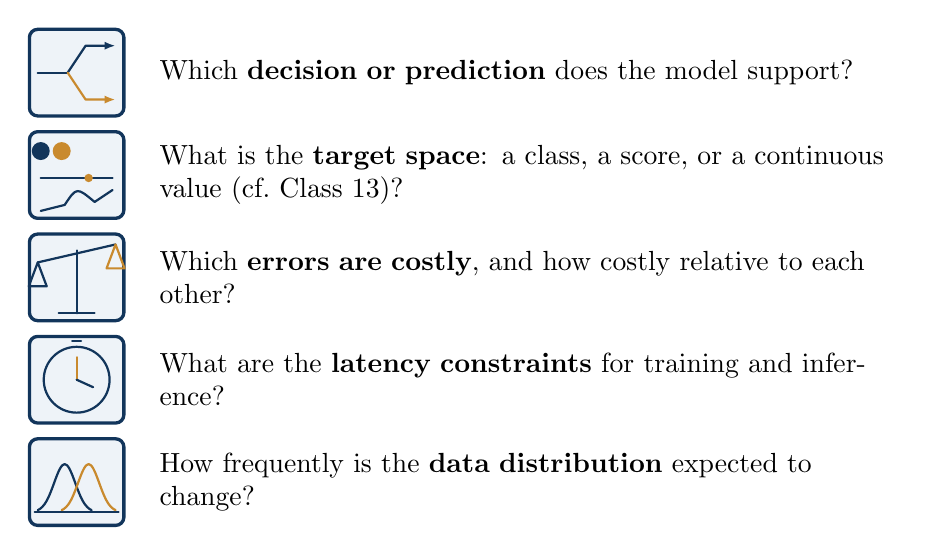
\begin{tikzpicture}
\foreach \i/\t in {
 1/{Which \textbf{decision or prediction} does the model support?},
 2/{What is the \textbf{target space}: a class, a score, or a continuous value (cf.\ Class 13)?},
 3/{Which \textbf{errors are costly}, and how costly relative to each other?},
 4/{What are the \textbf{latency constraints} for training and inference?},
 5/{How frequently is the \textbf{data distribution} expected to change?}}{
  \node[inner sep=0] (i\i) at (0,{-(\i-1)*1.3}) {\qicon{\i}};
  \node[anchor=west, text width=0.78\textwidth, align=left] at ([xshift=0.3cm]i\i.east) {\t};
}
\end{tikzpicture}
\coursefooter
\end{frame}

\qaslide{1}{decision or prediction}{Which decision or prediction does the model support?}
{An automatic action}
{\begin{itemize}
\item Example: label each bottle as premium or standard on the price list, with no human review.
\item The model must output a \textbf{reliable class (and probability)} the system can act on.
\item Favors models with reliable scores (logistic regression, gradient boosting) and a documented decision rule.
\end{itemize}}
{Support for a human}
{\begin{itemize}
\item Example: rank wines for a sommelier to taste first.
\item Only the \textbf{ordering} of cases matters, and the sommelier needs a reason for each ranking.
\item Favors ranking metrics (precision at $k$) and interpretable outputs.
\end{itemize}}

\qaslide{2}{target space}{What is the target space: a class, a score, or a continuous value?}
{A class}
{\begin{itemize}
\item Example: premium or standard wine (quality $\ge 7$ or not).
\item Use a \textbf{classifier}; optionally expose \texttt{predict\_proba} for a score.
\item Evaluate with precision, recall, and the confusion matrix, not with error in units.
\end{itemize}}
{A continuous value}
{\begin{itemize}
\item Example: the wine quality score itself; pasteurization temperature.
\item Use a \textbf{regressor}; the loss is measured in the units of the target.
\item Evaluate with MAE, RMSE, or $R^2$; the output is the answer itself.
\end{itemize}}

\qaslide{3}{costly errors}{Which errors are costly, and how costly relative to each other?}
{A missed positive is worse}
{\begin{itemize}
\item Example: a premium wine sold as standard loses its margin, which costs more than the opposite error.
\item Favor \textbf{recall}: use class weights or oversample the rare class.
\item Accept more false positives, and budget the returns or re-tastings they create.
\end{itemize}}
{A false alarm is worse}
{\begin{itemize}
\item Example: a standard wine sold as premium triggers returns and damages the brand.
\item Favor \textbf{precision}: label premium only on strong evidence.
\item Accept that some positives will be missed; make this explicit to the stakeholders.
\end{itemize}}

\qaslide{4}{latency}{What are the latency constraints for training and inference?}
{Strict, real-time inference}
{\begin{itemize}
\item Example: a response within milliseconds inside an API.
\item Favor \textbf{light models}: linear models, shallow trees, a small ensemble.
\item Preprocessing must be cheap, and the full \texttt{Pipeline} must be loaded once at start-up.
\end{itemize}}
{Offline, batch scoring}
{\begin{itemize}
\item Example: scoring every bottle of a new vintage in one batch.
\item Large ensembles and \textbf{extensive hyperparameter search} are affordable.
\item The limit is the total training budget, which must be tracked per run.
\end{itemize}}

\qaslide{5}{distribution change}{How frequently is the data distribution expected to change?}
{Stable distribution}
{\begin{itemize}
\item Example: a controlled laboratory measurement.
\item A \textbf{fixed model} retrained on a schedule is sufficient.
\item Monitor a few input statistics and the error, and register each retrained version.
\end{itemize}}
{Fast-changing distribution}
{\begin{itemize}
\item Example: a sensor stream with seasonal or process drift.
\item Favor \textbf{online or incremental models} and drift detection (Class 19).
\item Evaluate on the most recent data, not on a random split of the whole history.
\end{itemize}}

\begin{frame}{Model families in context: supervised learning}
\centering
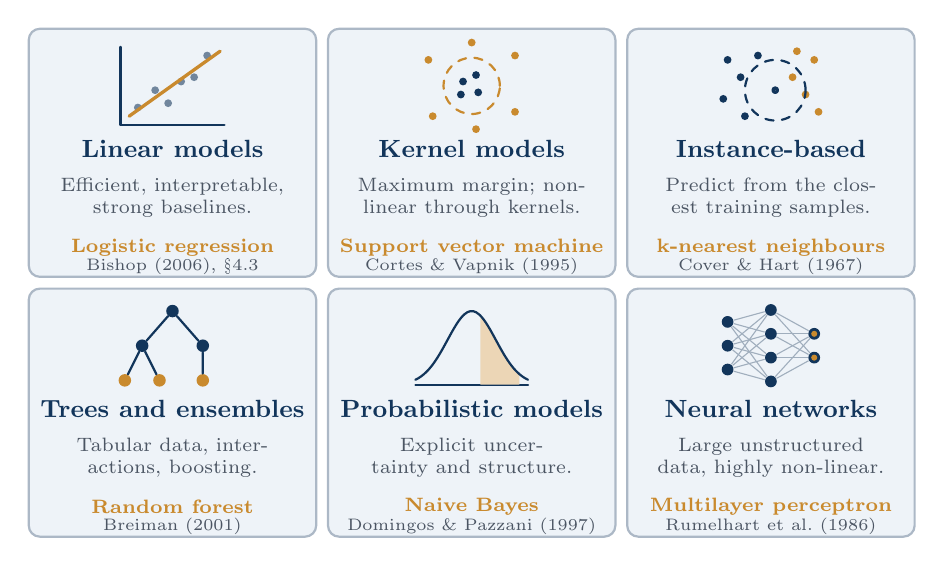
\begin{tikzpicture}
\famcard{0}{0}{1}{Linear models}{Efficient, interpretable, strong baselines.}{Logistic regression}{Bishop (2006), \S4.3}
\famcard{3.8}{0}{6}{Kernel models}{Maximum margin; non-linear through kernels.}{Support vector machine}{Cortes \& Vapnik (1995)}
\famcard{7.6}{0}{7}{Instance-based}{Predict from the closest training samples.}{k-nearest neighbours}{Cover \& Hart (1967)}
\famcard{0}{-3.3}{2}{Trees and ensembles}{Tabular data, interactions, boosting.}{Random forest}{Breiman (2001)}
\famcard{3.8}{-3.3}{3}{Probabilistic models}{Explicit uncertainty and structure.}{Naive Bayes}{Domingos \& Pazzani (1997)}
\famcard{7.6}{-3.3}{4}{Neural networks}{Large unstructured data, highly non-linear.}{Multilayer perceptron}{Rumelhart et al.\ (1986)}
\end{tikzpicture}
\coursefooter
\end{frame}

\begin{frame}{Model families in context: beyond the supervised toolbox}
\centering
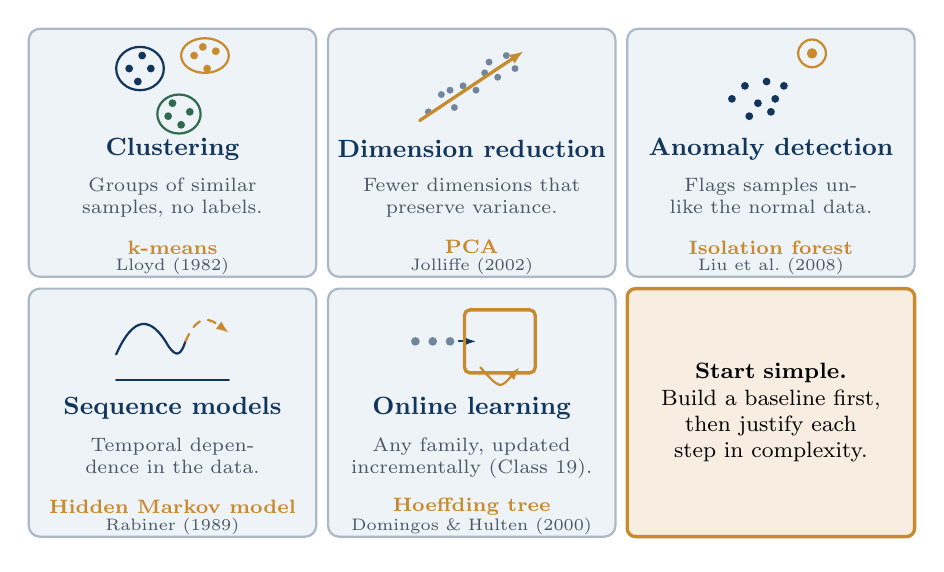
\begin{tikzpicture}
\famcard{0}{0}{8}{Clustering}{Groups of similar samples, no labels.}{k-means}{Lloyd (1982)}
\famcard{3.8}{0}{9}{Dimension reduction}{Fewer dimensions that preserve variance.}{PCA}{Jolliffe (2002)}
\famcard{7.6}{0}{10}{Anomaly detection}{Flags samples unlike the normal data.}{Isolation forest}{Liu et al.\ (2008)}
\famcard{0}{-3.3}{11}{Sequence models}{Temporal dependence in the data.}{Hidden Markov model}{Rabiner (1989)}
\famcard{3.8}{-3.3}{5}{Online learning}{Any family, updated incrementally (Class 19).}{Hoeffding tree}{Domingos \& Hulten (2000)}
\node[accentbox, minimum width=3.65cm, minimum height=3.15cm, text width=3.2cm, font=\footnotesize] at (7.6,-3.3) {\textbf{Start simple.}\\Build a baseline first, then justify each step in complexity.};
\end{tikzpicture}
\coursefooter
\end{frame}

\begin{frame}{scikit-learn as an architecture: one interface for every model}
\begin{tabularx}{\textwidth}{>{\bfseries}l >{\ttfamily}l X}
Estimator & fit(X, y) & Learns from data and stores the result in attributes ending with an underscore (e.g.\ \texttt{coef\_}). \\
\addlinespace[0.3em]
Predictor & predict(X) & Maps new samples to labels or values; classifiers also expose \texttt{predict\_proba}, and all predictors expose \texttt{score}. \\
\addlinespace[0.3em]
Transformer & transform(X) & Rewrites the features (scaling, encoding, imputation); \texttt{fit\_transform} is the shortcut for the training split. \\
\addlinespace[0.3em]
Meta-estimator & fit / predict & Wraps other estimators and exposes the same interface (\texttt{Pipeline}, \texttt{GridSearchCV}). \\
\bottomrule
\end{tabularx}
\coursefooter
\end{frame}

\begin{frame}[fragile]{The fit / predict contract}
\begin{lstlisting}[style=coursepython, columns=fixed, escapeinside={(*}{*)}]
from sklearn.ensemble import RandomForestClassifier
from sklearn.preprocessing import StandardScaler

scaler = StandardScaler().(*\hlcode{fit}*)(X_train)      # learns mean, s.d.
X_train_s = scaler.(*\hlcode{transform}*)(X_train)
X_test_s = scaler.(*\hlcode{transform}*)(X_test)         # same parameters

model = RandomForestClassifier(n_estimators=200, random_state=42)
model.(*\hlcode{fit}*)(X_train_s, y_train)               # learning happens here

y_pred = model.(*\hlcode{predict}*)(X_test_s)            # labels (tau = 0.5)
y_prob = model.(*\hlcode{predict_proba}*)(X_test_s)[:, 1]  # scores
\end{lstlisting}
\coursefooter
\end{frame}

\begin{frame}[fragile]{Pipeline: preprocessing and model as a single estimator}
\begin{lstlisting}[style=coursepython, columns=fixed, escapeinside={(*}{*)}]
from sklearn.pipeline import Pipeline
from sklearn.preprocessing import StandardScaler
from sklearn.linear_model import LogisticRegression
from sklearn.svm import SVC
from sklearn.ensemble import RandomForestClassifier
models = {
    "logistic": LogisticRegression(C=1.0, max_iter=1000),
    "svm": SVC(kernel="rbf", C=10, gamma="scale"),
    "forest": RandomForestClassifier(n_estimators=200, max_depth=8),
}
for name, clf in models.items():
    pipeline = Pipeline([("scaler", StandardScaler()),
                         ("model", clf)])
    pipeline.(*\hlcode{fit}*)(X_train, y_train)
    y_pred = pipeline.(*\hlcode{predict}*)(X_test)
\end{lstlisting}
\coursefooter
\end{frame}

\partslide{2}{Experiment tracking and search}{How do we compare models fairly and keep a record of every run?}{What to track, sources of bias, hyperparameter search, Weights \& Biases}

\begin{frame}{What must be tracked, and why}
\begin{tabularx}{\textwidth}{>{\bfseries}l X}
Dataset version or extraction date & Allows a result to be reproduced on the same data. \\
\addlinespace[0.3em]
Feature pipeline version & Separates the effect of preprocessing changes from that of model changes. \\
\addlinespace[0.3em]
Hyperparameters and random seeds & Identify the exact configuration that produced a result. \\
\addlinespace[0.3em]
Metrics, confusion matrices, artifacts & Allow the trained model, not only a number, to be audited. \\
\addlinespace[0.3em]
Code commit or notebook snapshot & Allows the logic behind a run to be replayed later (Class 17). \\
\bottomrule
\end{tabularx}
\coursefooter
\end{frame}

\begin{frame}{A fair comparison: hold everything else fixed}
\centering
\hyphenpenalty=10000 \exhyphenpenalty=10000
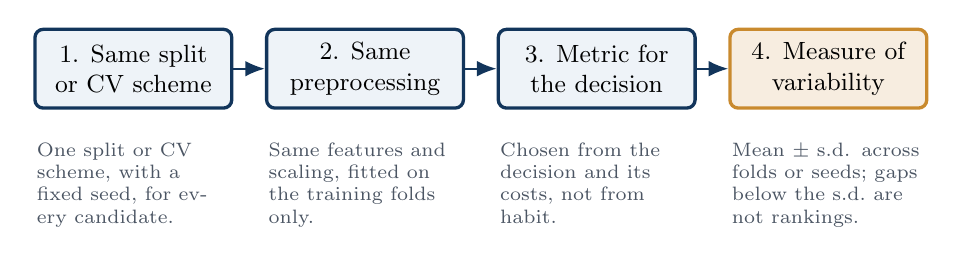
\begin{tikzpicture}[node distance=0.35cm and 0.4cm, font=\footnotesize]
\node[flowbox, minimum width=2.5cm, minimum height=1cm] (a) {1. Same split\\or CV scheme};
\node[flowbox, minimum width=2.5cm, minimum height=1cm, right=of a] (b) {2. Same\\preprocessing};
\node[flowbox, minimum width=2.5cm, minimum height=1cm, right=of b] (c) {3. Metric for\\the decision};
\node[accentbox, minimum width=2.5cm, minimum height=1cm, right=of c] (d) {4. Measure of\\variability};
\draw[arrow] (a) -- (b); \draw[arrow] (b) -- (c); \draw[arrow] (c) -- (d);
\foreach \n/\t in {
 a/{One split or CV scheme, with a fixed seed, for every candidate.},
 b/{Same features and scaling, fitted on the training folds only.},
 c/{Chosen from the decision and its costs, not from habit.},
 d/{Mean $\pm$ s.d. across folds or seeds; gaps below the s.d.\ are not rankings.}}{
  \node[below=0.3cm of \n, text width=2.45cm, align=left, font=\scriptsize, text=coursegray] {\t};
}
\end{tikzpicture}
\vspace{1.2cm}
\begin{block}{Why it matters}
A difference between two models is evidence only if the data, the preprocessing (unless preprocessing is the experiment), and the metric are identical, and if the difference exceeds the run-to-run variability.
\end{block}
\coursefooter
\end{frame}

\begin{frame}{Sources of bias and their solutions}
\begin{tabularx}{\textwidth}{>{\raggedright\arraybackslash}X >{\raggedright\arraybackslash}X}
\toprule
\textbf{\color{courseblue}Source of bias} & \textbf{\textcolor{coursegreen}{Solution}} \\
\midrule
\textbf{Test-set reuse.} Reusing the test set until it becomes part of tuning (model-selection leakage). & \textcolor{coursegreen}{Tune on a validation split or with cross-validation; use the test set once, at the end.} \\
\addlinespace[0.6em]
\textbf{Hidden state.} Hidden notebook state and untracked edits. & \textcolor{coursegreen}{Log commit, configuration, seed, and data version with every run; restart the kernel and run all cells.} \\
\addlinespace[0.6em]
\textbf{Selective reporting.} Reporting only the best run. & \textcolor{coursegreen}{Report all runs and the search budget; give mean $\pm$ s.d. over folds or seeds.} \\
\bottomrule
\end{tabularx}
\coursefooter
\end{frame}

\begin{frame}{Hyperparameter search strategies}
\begin{tabularx}{\textwidth}{>{\bfseries}l X}
Manual tuning & Small problems; useful to build intuition. \\
\addlinespace[0.3em]
Grid search & Exhaustive evaluation of a small, structured search space. \\
\addlinespace[0.3em]
Random search & Better coverage when only a few of many hyperparameters matter (Bergstra and Bengio, 2012). \\
\addlinespace[0.3em]
\multicolumn{2}{l}{\textbf{Optimization-based search:} the validation score is treated as a black-box function.} \\
\addlinespace[0.2em]
\hspace{1em}Bayesian optimization & A surrogate model of the score (Gaussian process, TPE) guides the next trial; suited to expensive models. \\
\addlinespace[0.2em]
\hspace{1em}Genetic algorithms & A population of configurations evolves through selection, crossover, and mutation. \\
\addlinespace[0.2em]
\hspace{1em}Other heuristics & Simulated annealing, particle swarm, and bandit-based early stopping (successive halving, Hyperband). \\
\bottomrule
\end{tabularx}
\coursefooter
\end{frame}

\begin{frame}{Case study: how much does tuning help a decision tree?}
\begin{minipage}[c]{0.12\textwidth}

\includegraphics[height=1.9cm]{images/class18_dmkd_cover.png}
\end{minipage}\hspace{0.02\textwidth}
\begin{minipage}[c]{0.84\textwidth}
{\scriptsize Mantovani, Horv\'ath, Rossi, Cerri, Barbon Junior, Vanschoren, de Carvalho (2024). \emph{Better trees: an empirical study on hyperparameter tuning of classification decision tree induction algorithms}. Data Mining and Knowledge Discovery, 38(3), 1364--1416.}
\end{minipage}
\vspace{0.2em}
\begin{columns}[T]
\column{0.48\textwidth}
\begin{block}{Experimental design}
\footnotesize
\begin{itemize}\setlength{\itemsep}{1pt}
\item \textbf{Models and data:} CART and C4.5; 94 OpenML classification datasets.
\item \textbf{Six techniques:} random search, genetic algorithm, particle swarm, estimation of distribution, model-based optimization, Irace.
\item \textbf{Protocol:} nested CV (10 outer, 3 inner folds); same partitions and seeds; 900 evaluations.
\item \textbf{Baseline:} default hyperparameters.
\end{itemize}
\end{block}
\column{0.48\textwidth}
\begin{alertblock}{Findings}
\footnotesize
\begin{itemize}\setlength{\itemsep}{1pt}
\item Significant gains over the defaults: \textbf{CART} in about two thirds of the datasets, \textbf{C4.5} in one third.
\item \textbf{Irace} was the best technique; few evaluations were enough.
\item \textbf{A small subset of hyperparameters} explains most of the gain (CART: \texttt{minsplit}, \texttt{minbucket}).
\item \textbf{Defaults can already be good}.
\end{itemize}
\end{alertblock}
\end{columns}
\coursefooter
\end{frame}

\begin{frame}{What is Weights \& Biases (W\&B)?}
\begingroup\footnotesize
A platform for \textbf{tracking, comparing, and versioning machine learning work}. A few lines of the \texttt{wandb} Python library send metrics, configuration, and files to a web dashboard, which can be hosted by W\&B or self-hosted. Website: \href{https://wandb.ai}{wandb.ai}.
\vspace{0.5em}

\begin{tabularx}{\textwidth}{>{\bfseries}l X}
Run & One execution of a script or notebook, with a unique identifier. \\
\addlinespace[0.3em]
Config & The inputs of a run: hyperparameters, seed, dataset version. \\
\addlinespace[0.3em]
Metrics & Values logged with \texttt{run.log}: scores, losses, timings, plots. \\
\addlinespace[0.3em]
Sweep & An automated hyperparameter search (grid, random, or Bayesian). \\
\addlinespace[0.3em]
Artifact & A versioned file or directory (dataset, model) with its lineage. \\
\addlinespace[0.3em]
Registry & Curated collections of approved model versions. \\
\bottomrule
\end{tabularx}
\par\endgroup
\vspace{0.5em}
\begin{block}{In one sentence}
\footnotesize Git remembers how the code changed; W\&B remembers what each run of that code produced.
\end{block}
\vspace{0.3em}
{\scriptsize \textbf{Alternatives:} \href{https://mlflow.org}{MLflow} (open source, self-hosted), \href{https://www.tensorflow.org/tensorboard}{TensorBoard} (local dashboards), \href{https://www.comet.com}{Comet}, \href{https://clear.ml}{ClearML}.\par}
\coursefooter
\end{frame}

\begin{frame}{W\&B case study: search space and protocol}
\begin{columns}[T]
\column{0.5\textwidth}
\begingroup\footnotesize
\textbf{Search space} of a gradient boosting regressor:
\vspace{0.3em}

\begin{tabular}{>{\ttfamily}l l}
\normalfont\bfseries Hyperparameter & \bfseries Values \\
\toprule
n\_estimators & 100, 200, 300 \\
max\_depth & 3, 5, 7 \\
learning\_rate & 0.05, 0.1, 0.2 \\
min\_samples\_split & 2, 5, 10 \\
\bottomrule
\end{tabular}
\par\endgroup
\column{0.48\textwidth}
\begingroup\footnotesize
\textbf{Protocol:}
\begin{itemize}
\item Data: red wine quality, 1{,}599 samples; target \texttt{quality}.
\item Split: 75\% training (1{,}199 wines), 25\% test (400 wines), fixed seed.
\item Grid search: $3^4 = 81$ configurations (one W\&B run each) $\times$ 5-fold cross-validation $=$ 405 fits, scored by $R^2$ on the training split; each run then refits once to save its artifact.
\item The test split is used once, after selection.
\end{itemize}
\par\endgroup
\end{columns}
\vspace{0.6em}
{\scriptsize Implemented in the \texttt{wine-wandb} project (\texttt{configs/sweep.yaml}, \texttt{src/wine\_wandb/sweep.py}); no numerical result of the sweep is shown until it has been executed.\par}
\coursefooter
\end{frame}

\begin{frame}{W\&B: the record behind an experiment}
\begingroup\footnotesize
The experiment tracker links an explicit hypothesis to a reproducible configuration and measurable evidence. An example record for the wine-quality exercise:
\vspace{0.4em}
\begin{tabularx}{\textwidth}{>{\ttfamily}l X}
\normalfont\bfseries Field & \bfseries Example logged information \\
\toprule
run.config & model family, grid, random seed, cross-validation scheme \\
run.summary & mean CV $R^2$, CV standard deviation, fitting time \\
git commit & commit SHA for training and preprocessing code \\
dataset & dataset identifier, checksum or immutable artifact version \\
model artifact & serialized \texttt{Pipeline} (preprocessing + predictor) \\
\bottomrule
\end{tabularx}
\par\endgroup
\vspace{0.5em}
\begin{itemize}\footnotesize
\item Log candidate performance using cross-validation on the training partition; evaluate the chosen model only once on the untouched test partition.
\item \textbf{Do not confuse} experiment logs, artifact versions, and model approval: they answer different questions.
\end{itemize}
\coursefooter
\end{frame}

\begin{frame}[fragile]{W\&B: minimal experiment tracking in Python}
\begin{lstlisting}[style=coursepython, columns=fixed, escapeinside={(*}{*)}]
import wandb
from sklearn.model_selection import cross_val_score

config = {"model": "GradientBoostingRegressor", "seed": 42}
with (*\hlcode{wandb.init}*)(project="wine-quality", config=config) as run:
    scores = cross_val_score(pipeline, X_train, y_train, cv=5)
    run.(*\hlcode{log}*)({"cv/r2_mean": scores.mean(),
             "cv/r2_std": scores.std()})
    artifact = wandb.(*\hlcode{Artifact}*)("wine-pipeline", type="model")
    artifact.add_file("pipeline.joblib")
    run.(*\hlcode{log\_artifact}*)(artifact)
\end{lstlisting}
\coursefooter
\end{frame}

\partslide{3}{Artifacts, versioning, and registry}{How does a trained model become an approved, versioned, reversible release?}{Git versus artifacts, the W\&B Registry, promotion and rollback}

\begin{frame}{Git, tracking, artifacts, and registry: distinct roles}
\begingroup\footnotesize
\begin{tabularx}{\textwidth}{>{\bfseries}l X X}
Component & Stores or identifies & Primary question \\
\toprule
GitHub & source, tests, configuration, CI workflows & Which code produced this run? \\
W\&B Runs & parameters, metrics, environment and run identifiers & What happened during training? \\
W\&B Artifacts & immutable versions of data and model files & Which exact file was produced or used? \\
W\&B Registry & curated collections and approved model versions & Which version is eligible for operational use? \\
\bottomrule
\end{tabularx}
\par\endgroup
\vspace{0.6em}
\begin{block}{Key distinction}
\footnotesize Versioning a \texttt{model.pkl} filename is not enough: a deployed model needs \emph{code + data + preprocessing + environment + trained artifact + approval record}.
\end{block}
\coursefooter
\end{frame}

\begin{frame}{Why not commit trained binaries directly to Git?}
\begin{columns}[T]
\column{0.49\textwidth}
\textbf{Git is excellent for}\begin{itemize}\footnotesize
\item code and configuration diffs;
\item review and pull requests;
\item reproducible workflow definitions.
\end{itemize}
\column{0.49\textwidth}
\textbf{Model artifacts additionally need}\begin{itemize}\footnotesize
\item versioned object storage and integrity hashes;
\item links to runs and input datasets;
\item approval, access control, and rollback history.
\end{itemize}
\end{columns}
\vspace{0.5em}
\begin{block}{Practical exception}
\footnotesize Tiny demonstration binaries may be committed for a self-contained example, but this is not a scalable production artifact strategy. Git LFS manages large files differently; it does not by itself provide experiment tracking or model governance.
\end{block}
\coursefooter
\end{frame}

\begin{frame}{From an experiment to an approved model}
\centering
\definecolor{deploycolor}{HTML}{7A4E9C}
\begin{tikzpicture}[node distance=0.45cm and 0.55cm, font=\scriptsize,
  gitbox/.style={flowbox, draw=courseblue, fill=courseblue!12, minimum width=2.1cm},
  wandbbox/.style={flowbox, draw=coursegold, fill=coursegold!18, minimum width=2.1cm},
  serverbox/.style={flowbox, draw=coursegreen, fill=coursegreen!14, minimum width=2.1cm},
  deploybox/.style={flowbox, draw=deploycolor, fill=deploycolor!12, minimum width=2.1cm},
  legend/.style={rounded corners=2pt, very thick, minimum width=2.4cm, minimum height=0.5cm, font=\scriptsize}]
\node[gitbox] (git) {Git commit\\code + config};
\node[serverbox, right=of git] (train) {Training run\\executed on the server};
\node[wandbbox, right=of train] (compare) {Validation\\compare candidates};
\node[wandbbox, below=0.8cm of compare] (artifact) {Versioned artifact\\model + metadata};
\node[wandbbox, left=of artifact] (registry) {Registry\\approval + alias};
\node[deploybox, left=of registry] (serve) {Application\\load selected version};
\draw[arrow] (git) -- (train);
\draw[arrow] (train) -- (compare);
\draw[arrow] (compare) -- (artifact);
\draw[arrow] (artifact) -- (registry);
\draw[arrow] (registry) -- (serve);
\draw[arrow, dashed] (git.south) -- (serve.north);
\node[legend, draw=courseblue, fill=courseblue!12, below=0.7cm of serve, xshift=-0.4cm] (l1) {Git};
\node[legend, draw=coursegold, fill=coursegold!18, right=0.3cm of l1] (l2) {W\&B};
\node[legend, draw=coursegreen, fill=coursegreen!14, right=0.3cm of l2] (l3) {Execution server};
\node[legend, draw=deploycolor, fill=deploycolor!12, right=0.3cm of l3] (l4) {Deploy (possible)};
\end{tikzpicture}
\coursefooter
\end{frame}

\begin{frame}[fragile]{W\&B: publish an artifact to the Registry}
\begin{lstlisting}[style=coursepython, columns=fixed, escapeinside={(*}{*)}]
import wandb
import joblib

joblib.dump(pipeline, "pipeline.joblib")
with wandb.init(project="wine-quality") as run:
    artifact = wandb.(*\hlcode{Artifact}*)("wine-pipeline", type="model")
    artifact.(*\hlcode{add\_file}*)("pipeline.joblib")
    logged = run.(*\hlcode{log\_artifact}*)(artifact)
    logged.wait()
    run.link_artifact(
        logged,
        target_path="wandb-registry-model/wine-quality",
    )
\end{lstlisting}
\coursefooter
\end{frame}

\begin{frame}{Promotion, rollback, and a model release contract}
\begin{enumerate}\footnotesize
\item \textbf{Candidate:} compare runs on validation data; preserve the full candidate record.
\item \textbf{Gate:} test metrics, stability, inference latency, feature schema, and reproducibility against agreed criteria.
\item \textbf{Approval:} link the accepted artifact to a Registry collection; assign a documented alias such as \texttt{champion} when appropriate.
\item \textbf{Release:} application records the resolved immutable artifact version and environment.
\item \textbf{Rollback:} repoint the release to the preceding approved artifact and revalidate compatibility.
\end{enumerate}
\begin{block}{Discussion}
\footnotesize Why is selecting the highest CV score insufficient to promote a model to production?
\end{block}
\coursefooter
\end{frame}

\partslide{4}{Evaluation}{Which metric tells the truth about this task?}{Metrics, class imbalance, inspecting the errors}

\begin{frame}{Evaluation metrics must match the task}
{\small Tracking identifies which run performed best; it does not establish whether that run is adequate for the decision it supports.\par}
\vspace{0.3em}
\begin{columns}[T]
\column{0.49\textwidth}
\begin{block}{Classification (premium wine)}
\footnotesize
\begin{itemize}\setlength{\itemsep}{2pt}
\item \textbf{Precision} $=\frac{TP}{TP+FP}$ and \textbf{recall} $=\frac{TP}{TP+FN}$, from the counts of true and false positives and negatives.
\item \textbf{PR-AUC:} area under the precision--recall curve; summarizes all possible cut-offs.
\item \textbf{Accuracy} alone is misleading when classes are imbalanced.
\item \textbf{Calibration:} needed when an action depends on the predicted probability.
\end{itemize}
\end{block}
\column{0.49\textwidth}
\begin{alertblock}{Regression (wine quality)}
\footnotesize
\begin{itemize}\setlength{\itemsep}{2pt}
\item \textbf{MAE} $=\frac{1}{n}\sum_i |y_i-\hat{y}_i|$ and \textbf{RMSE} $=\sqrt{\frac{1}{n}\sum_i (y_i-\hat{y}_i)^2}$, in the unit of the target (quality points).
\item \textbf{RMSE} penalizes large errors more than MAE does.
\item \textbf{$R^2$:} share of the variance explained; 0 for a model that always predicts the mean.
\item \textbf{Residuals} show where the model fails, for example at extreme scores.
\end{itemize}
\end{alertblock}
\end{columns}
\coursefooter
\end{frame}

\begin{frame}{The wine dataset at a glance}
\centering
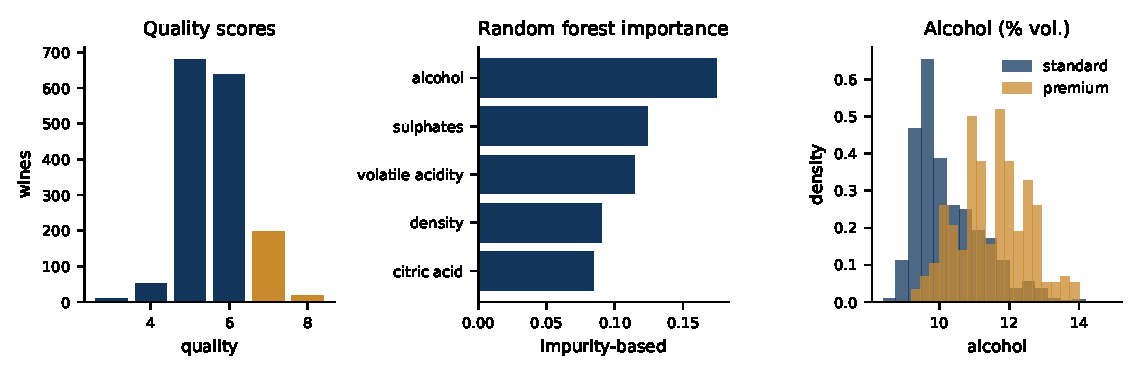
\includegraphics[width=\textwidth,height=0.46\textheight,keepaspectratio]{images/class18_wine_overview.pdf}

\vspace{0.3em}
\begin{itemize}\footnotesize
\item \textbf{Imbalance:} 217 of 1{,}599 wines (13.6\%) have quality $\ge 7$ and are labelled \emph{premium}; the same split as the regression exercise gives 1{,}199 training and 400 test wines (164 and 53 premium).
\item \textbf{Importance:} alcohol, sulphates, and volatile acidity account for 41\% of the impurity-based importance of the random forest; importance measures association, not causal effect.
\item \textbf{Separation:} premium wines have a higher median alcohol content (11.6 versus 10.0\% vol.), but the distributions overlap, so no single feature decides the label.
\end{itemize}
\coursefooter
\end{frame}

\begin{frame}{Inspecting the errors}
\begin{columns}[T]
\column{0.42\textwidth}
\centering
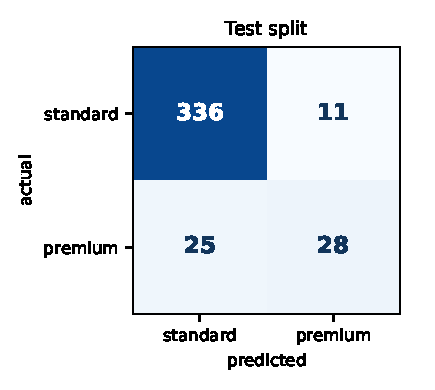
\includegraphics[width=0.95\linewidth]{images/class18_wine_confusion_matrix.pdf}

{\scriptsize Test split (400 wines), random forest, predicted classes.\par}
\column{0.56\textwidth}
\begingroup\footnotesize
\[
\text{precision} = \frac{28}{28 + 11} = 0.72, \qquad \text{recall} = \frac{28}{28 + 25} = 0.53
\]
\[
\text{accuracy} = \frac{336 + 28}{400} = 0.91
\]
\par\endgroup
\begin{itemize}\footnotesize
\item 25 of the 53 premium wines are missed (FN), while 11 standard wines are labelled premium (FP).
\item The accuracy of 91\% sounds good, but always answering ``standard'' already scores 86.75\%; the confusion matrix exposes the missed premium wines.
\item Whether 25 missed wines are acceptable depends on the cost of a missed premium wine relative to a wrong label: a business input, not a property of the model.
\end{itemize}
\end{columns}
\coursefooter
\end{frame}

\begin{frame}{Accuracy fails under imbalance: alternatives}
\begin{block}{Wine example}
\footnotesize Always answering ``standard'' scores 86.75\% accuracy with a recall of 0. The random forest reaches 91\%, only 4 points more, yet misses almost half of the premium wines.
\end{block}
\begingroup\footnotesize
\begin{tabularx}{\textwidth}{>{\bfseries}l >{\raggedright\arraybackslash}X r r}
Metric & What it measures & Always ``standard'' & Random forest \\
\toprule
Accuracy & Share of correct answers; dominated by the majority class. & 0.87 & 0.91 \\
F1-score & Harmonic mean of precision and recall, $2PR/(P+R)$; ignores true negatives. & 0 & 0.61 \\
ROC-AUC & Chance that a random premium wine outscores a random standard one; independent of any cut-off. & 0.50 & 0.94 \\
PR-AUC & Area under the precision--recall curve; chance level is the share of positives. & 0.13 & 0.75 \\
\bottomrule
\end{tabularx}
\par\endgroup
\vspace{0.3em}
\begin{itemize}\footnotesize
\item F1 is computed from the predicted classes and weighs both errors equally.
\item ROC-AUC (0.94) exceeds PR-AUC (0.75) because true negatives dominate; with rare positives, prefer PR-AUC.
\item None encodes the cost of each error: that is a business input.
\end{itemize}
\coursefooter
\end{frame}

\partslide{5}{From prediction to decision}{How does a score become an action that people can trust?}{Interfaces, the decision rule, decision support, where trust breaks}

\begin{frame}{A registered model creates value through an interface}
\begin{itemize}
\item A registered trained model that cannot be invoked or interpreted has limited practical value, regardless of its offline metrics.
\item An interface makes predictions available to users, services, and operational workflows.
\item The interface also determines trust: input validation, response format, and clarity matter as much as the metric used to select the model.
\end{itemize}
\coursefooter
\end{frame}

\begin{frame}{A prediction is not a decision}
\begin{itemize}
\item A premium score suggests that a wine deserves a tasting, not a final grade; a process alert suggests investigation, not automatic shutdown.
\item A classifier estimates $P(y = 1 \mid \mathbf{x})$; the class it outputs applies a decision rule, $\hat{y} = \mathbf{1}[\hat{p}(\mathbf{x}) \ge 0.5]$.
\item \texttt{predict} makes that rule implicit: it assumes both errors cost the same.
\end{itemize}
\begin{block}{In this class}
We adopt the predicted class as the decision. With unequal error costs, the cut-off would be a separate design choice.
\end{block}
\coursefooter
\end{frame}

\begin{frame}{Example: a decision-support interface for wine}
\centering
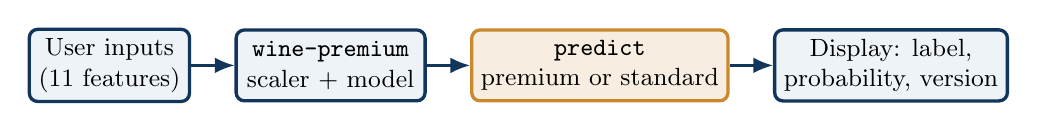
\begin{tikzpicture}[node distance=0.55cm, font=\footnotesize]
\node[flowbox, minimum width=1.9cm] (in) {User inputs\\(11 features)};
\node[flowbox, minimum width=2.4cm, right=of in] (sc) {\texttt{wine-premium}\\scaler + model};
\node[accentbox, minimum width=2.1cm, right=of sc] (p) {\texttt{predict}\\premium or standard};
\node[flowbox, minimum width=2.6cm, right=of p] (out) {Display: label,\\probability, version};
\draw[arrow] (in) -- (sc); \draw[arrow] (sc) -- (p); \draw[arrow] (p) -- (out);
\end{tikzpicture}
\vspace{0.6em}
\begin{itemize}\footnotesize
\item The interface loads the registered \texttt{wine-premium} artifact, so preprocessing cannot diverge from training, and shows the predicted label together with the estimated probability.
\item The predicted class is the decision; the probability tells the user how confident the model is.
\item The interface should identify the exact artifact version it loaded.
\end{itemize}
\coursefooter
\end{frame}

\begin{frame}{A decision-support interface: requirements and failure modes}
\begin{columns}[T]
\column{0.49\textwidth}
\begin{block}{What it must provide}
\footnotesize
\begin{itemize}\setlength{\itemsep}{2pt}
\item What the model does and does not do.
\item Inputs that are meaningful domain variables, not technical internals.
\item Outputs that support action: label, probability, explanation.
\item Provenance: data version, model artifact version, monitoring signals.
\end{itemize}
\end{block}
\column{0.49\textwidth}
\begin{alertblock}{Where trust breaks down}
\footnotesize
\begin{itemize}\setlength{\itemsep}{2pt}
\item Uncertainty hidden behind one precise-looking number.
\item Inputs that violate the assumptions of training.
\item A decision rule adopted by default and never revisited.
\item A demonstration model that looks authoritative without validation.
\end{itemize}
\end{alertblock}
\end{columns}
\coursefooter
\end{frame}

\partslide{6}{Practice and wrap-up}{How do the pieces fit together in a real repository?}{Repository connections and take-away}

\begin{frame}{Repository connections}
\repoactivity{
\begin{itemize}
\item The \texttt{wine-wandb} project (a separate repository): the complete wine-quality project used throughout this class, with two tasks on the same dataset.
\item \texttt{configs/}: \texttt{baseline.yaml} and \texttt{sweep.yaml} (regression), \texttt{classifier.yaml} (premium wine).
\item \texttt{train.py}, \texttt{sweep.py} and \texttt{train\_classifier.py}: tracked runs; each logs the dataset checksum, the Git commit, and a pipeline artifact (\texttt{wine-pipeline}, \texttt{wine-premium}).
\item \texttt{evaluate.py}, \texttt{register.py}, \texttt{figures.py}: one-time test evaluation, registry promotion, and the figures of this class.
\end{itemize}
}
\coursefooter
\end{frame}

\begin{frame}{Papers and materials}
\readinglist{
\fontsize{6.8}{8.2}\selectfont
\begin{columns}[T]
\column{0.5\textwidth}
\begin{itemize}\setlength{\itemsep}{1pt}
\item Bergstra, J., Bengio, Y. (2012). Random search for hyper-parameter optimization. \emph{Journal of Machine Learning Research}, 13, 281--305.
\item Bergstra, J., Yamins, D., Cox, D. (2013). Making a science of model search: Hyperparameter optimization in hundreds of dimensions for vision architectures. \emph{Proceedings of ICML}, PMLR 28(1), 115--123.
\item Bishop, C. M. (2006). \emph{Pattern Recognition and Machine Learning}. Springer.
\item Saito, T., Rehmsmeier, M. (2015). The precision-recall plot is more informative than the ROC plot when evaluating binary classifiers on imbalanced datasets. \emph{PLoS ONE}, 10(3), e0118432.
\item Mantovani, R. G., Horv\'ath, T., Rossi, A. L. D., Cerri, R., Barbon Junior, S., Vanschoren, J., de Carvalho, A. C. P. L. F. (2024). Better trees: an empirical study on hyperparameter tuning of classification decision tree induction algorithms. \emph{Data Mining and Knowledge Discovery}, 38(3), 1364--1416.
\item Niculescu-Mizil, A., Caruana, R. (2005). Predicting good probabilities with supervised learning. \emph{Proceedings of ICML}, 625--632.
\end{itemize}
\column{0.5\textwidth}
\begin{itemize}\setlength{\itemsep}{1pt}
\item Domingos, P. (2012). A few useful things to know about machine learning. \emph{Communications of the ACM}, 55(10), 78--87.
\item Hastie, T., Tibshirani, R., Friedman, J. (2009). \emph{The Elements of Statistical Learning} (2nd ed.). Springer.
\item Huyen, C. (2022). \emph{Designing Machine Learning Systems}. O'Reilly.
\item scikit-learn User Guide: \href{https://scikit-learn.org/stable/modules/grid_search.html}{tuning hyperparameters}; \href{https://scikit-learn.org/stable/modules/model_evaluation.html}{model evaluation}.
\item Tool documentation: \href{https://docs.wandb.ai/}{Weights \& Biases}; \href{https://mlflow.org/docs/latest/index.html}{MLflow}.
\end{itemize}
\end{columns}
}
\coursefooter
\end{frame}

\begin{frame}{Papers and materials: model families}
\readinglist{
\fontsize{6.8}{8.2}\selectfont
\begin{columns}[T]
\column{0.5\textwidth}
\begin{itemize}\setlength{\itemsep}{1pt}
\item Bishop, C. M. (2006). \emph{Pattern Recognition and Machine Learning}. Springer. (Logistic regression: \S4.3.)
\item Breiman, L. (2001). Random forests. \emph{Machine Learning}, 45(1), 5--32.
\item Cortes, C., Vapnik, V. (1995). Support-vector networks. \emph{Machine Learning}, 20(3), 273--297.
\item Cover, T., Hart, P. (1967). Nearest neighbor pattern classification. \emph{IEEE Transactions on Information Theory}, 13(1), 21--27.
\item Domingos, P., Pazzani, M. (1997). On the optimality of the simple Bayesian classifier under zero-one loss. \emph{Machine Learning}, 29, 103--130.
\item Friedman, J. H. (2001). Greedy function approximation: a gradient boosting machine. \emph{Annals of Statistics}, 29(5), 1189--1232.
\end{itemize}
\column{0.5\textwidth}
\begin{itemize}\setlength{\itemsep}{1pt}
\item Jolliffe, I. T. (2002). \emph{Principal Component Analysis} (2nd ed.). Springer.
\item Liu, F. T., Ting, K. M., Zhou, Z.-H. (2008). Isolation forest. \emph{Proceedings of ICDM}, 413--422.
\item Lloyd, S. P. (1982). Least squares quantization in PCM. \emph{IEEE Transactions on Information Theory}, 28(2), 129--137.
\item Rabiner, L. R. (1989). A tutorial on hidden Markov models and selected applications in speech recognition. \emph{Proceedings of the IEEE}, 77(2), 257--286.
\item Domingos, P., Hulten, G. (2000). Mining high-speed data streams. \emph{Proceedings of KDD}, 71--80.
\item Rumelhart, D. E., Hinton, G. E., Williams, R. J. (1986). Learning representations by back-propagating errors. \emph{Nature}, 323, 533--536.
\end{itemize}
\end{columns}
}
\coursefooter
\end{frame}

\begin{frame}{Take-away message}
\vfill
\centering
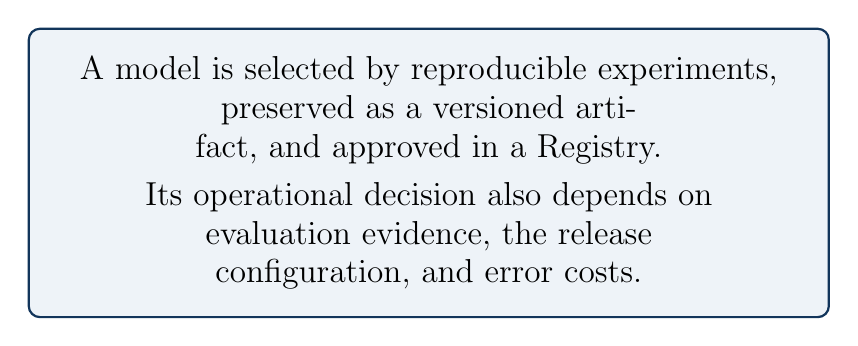
\begin{tikzpicture}
\node[fill=courseice, draw=courseblue, thick, rounded corners=4pt, inner sep=10pt, text width=0.78\textwidth, align=center, font=\large] {A model is selected by reproducible experiments,\\ preserved as a versioned artifact, and approved in a Registry.\\[0.3em] Its operational decision also depends on\\ evaluation evidence, the release configuration, and error costs.};
\end{tikzpicture}

\vfill
{\Large\bfseries\color{courseblue} Thank you for your attention.}

\vspace{0.4em}
{\small\color{coursegray} Next: Class 19 --- online machine learning and concept drift.}
\vfill
\coursefooter
\end{frame}

\end{document}
